\chapter{Datapath and Control}
\graphicspath{ {./chapter08/FigWork} }

%%%%%%%%%%%%%%%%%%%%%%%%%%%%%%%%%%%%%%%%%%%%%%%%%%%%
%% Here are the helpful stuff
%%%%%%%%%%%%%%%%%%%%%%%%%%%%%%%%%%%%%%%%%%%%%%%%%%%%
\section{Helpful Stuff}

\scalebox{0.7}{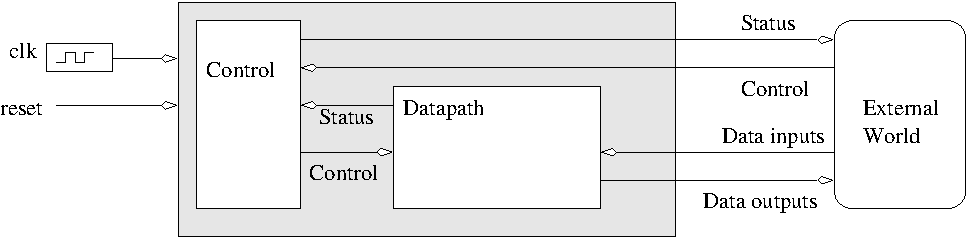
\includegraphics{../Fig/Abstract}}

Mini-C statements
\begin{itemize}
    \item if (condition) then BODY$_1$ else BODY$_2$
    \item for (i=A; i$<$B; i $+=$ 1) BODY
    \item while(condition) BODY
    \item X = value
\end{itemize}
where BODY contains 0 or more statements.
\vspace{0.1in}

\begin{tabular}{|l|l|l|l|l|} \hline
    Device      & Data in     & Data out & Status   & Control \\ \hline
    N:M Decoder &  1 bit       & M bits  &     & N bits  \\ \hline
    N:1 Mux     & N bits  & 1 bit    &     &  $\log_2(N)$ bits  \\ \hline
    MxNx1 Mux   & N, each M bits  & M bits &     &  $\log_2(N)$ bits  \\ \hline
    N bit adder &  2, each N bits & N bits & Overflow &   \\ \hline
    N bit add/sub & 2, each N bits & N bits & Overflow & 1 bit  \\ \hline
    N bit comparator  & 2, each N bits &  & 3 bits &   \\ \hline
    BCD to 7-segment  & 4-bits & 7-bits & &   \\ \hline
    N-bit priority encoder   & N-bits & $\log(N)$-bits & &   \\ \hline
    N bit register      & N bits & N bits &  & 1 bit  \\ \hline
    N bit shift register &  N bits & N bits &  & 2 bits  \\ \hline
    N bit counter       & N bits & N bits &  & 2 bits  \\ \hline
    Three state buffer    & N bits & N bits & & 1 bit  \\ \hline
    N:M RAM             & $\log_2(N)$ bits, M bits & M bit & & 2 bits  \\ \hline
    N-bit Bus transceiver     & N bits & N bits & & 2 bit  \\ \hline
\end{tabular}
\label{page:boxlist}

%%%%%%%%%%%%%%%%%%%%%%%%%%%%%%%%%%%%%%%%%%%%%%%%%%%%
%% Here are terms that the students define
%%%%%%%%%%%%%%%%%%%%%%%%%%%%%%%%%%%%%%%%%%%%%%%%%%%%
%%% \subsection{Definitions}
%%% \begin{description}
%%% \item [Control Word]
%%% \item [Status Word]
%%% \item[Two-line handshake]
%%% \end{description}

\begin{tabular}{|l|l|} \hline
    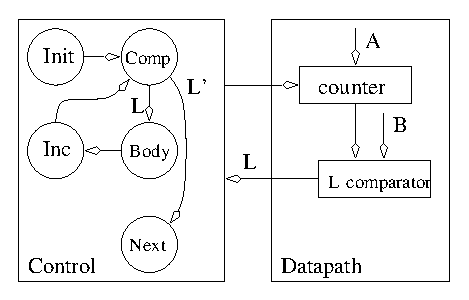
\includegraphics{../Fig/For}    & 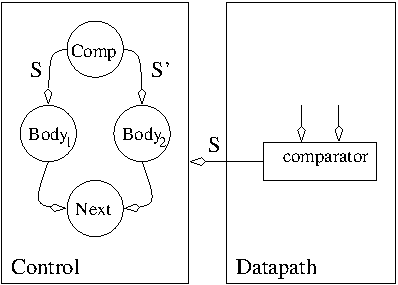
\includegraphics{../Fig/IfThen}      \\
    \verb-for(i=A; i<B; i++) BODY-  & \verb+if(condition) BODY1 else BODY2+\\ \hline

    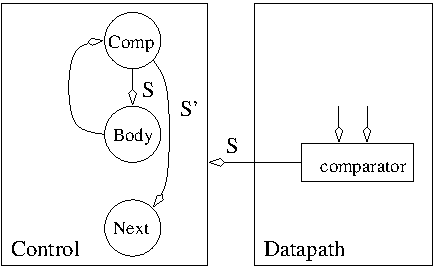
\includegraphics{../Fig/While}    & 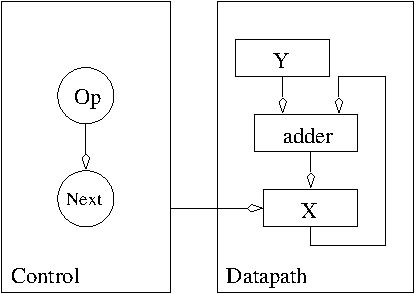
\includegraphics{../Fig/Op}    \\
    \verb+while(condition} BODY+    & \verb+x=value+         \\ \hline
\end{tabular}

%%%%%%%%%%%%%%%%%%%%%%%%%%%%%%%%%%%%%%%%%%%%%%%%%%%%
%% Here are the problems
%%%%%%%%%%%%%%%%%%%%%%%%%%%%%%%%%%%%%%%%%%%%%%%%%%%%
\section{Problems}
\begin{description}

    \item[Minimum Search]

        Design a digital circuit that looks for the smallest
        8-bit integer in a 128x8 bit RAM.  The numbers
        are stored at addresses $0\ldots 99$, you may assume that the
        RAM is preloaded with data.

\begin{verbatim}
1.  min = 0xFF;               // Set the min reg to largest value
2.  for (i=0; i<100; i++) {   // Search through the entire array
3.      MBR=RAM[i];           // read an 8-bit value from the RAM
4.      if (MBR<min) then     // If MBR is smaller than min
5.          min = MBR;        //   then set min to the smallest value
6   } // end for
\end{verbatim}

        \scalebox{0.7}{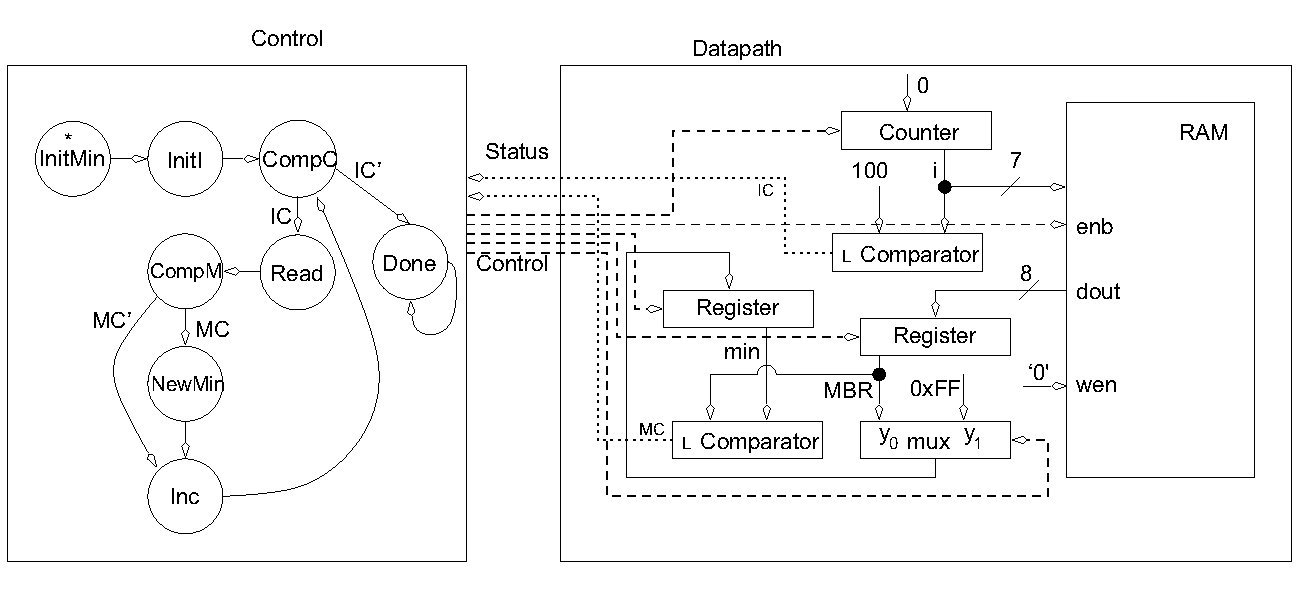
\includegraphics{../Fig/MinSearch}}

        \begin{tabular}{c||c|c|c|c|c}
            State   & enb       &  Reg Min  & Min mux       & Counter & MBR    \\ \hline
            & 0     &  0 hold   & 0 load FF     & 00 hold & 0 hold    \\ \hline
            & 1 read  &  1 load   & 1 load MBR    & 01 load & 1 load    \\ \hline
            &                 &           &               & 10 count&         \\ \hline
            &                &           &               & 11 reset& \\ \hline \hline
            InitMin &            &          &              &       &    \\ \hline
            InitI   &              &          &              &       &    \\ \hline
            CompC   &             &          &              &       &    \\ \hline
            Read    &             &          &              &       &    \\ \hline
            CompM   &           &          &              &       &    \\ \hline
            NewMin  &             &          &              &       &    \\ \hline
            Inc     &             &          &              &       &    \\ \hline
            Done    &             &          &              &       &    \\
        \end{tabular}

        \begin{tabular}{p{2in}p{1in}}
            $D_{IM} =$    &    $Z_{ENB} =$          \\
            $D_{II} =$     &    $Z_{RM} =$         \\
            $D_{CC} =$    &    $Z_{MM} =$          \\
            $D_{R} = $    &    $Z_{C1} =$         \\
            $D_{CM} =$     &    $Z_{C0} =$         \\
            $D_{NM} =$     &    $Z_{MBR} =$         \\
            $D_{I} = $    &             \\
            $D_{D} = $    &            \\
        \end{tabular}

        \pagebreak
        Shade the active FF and any BBBs which are read or written.

        \begin{tabular}{ll}
            \scalebox{0.3}{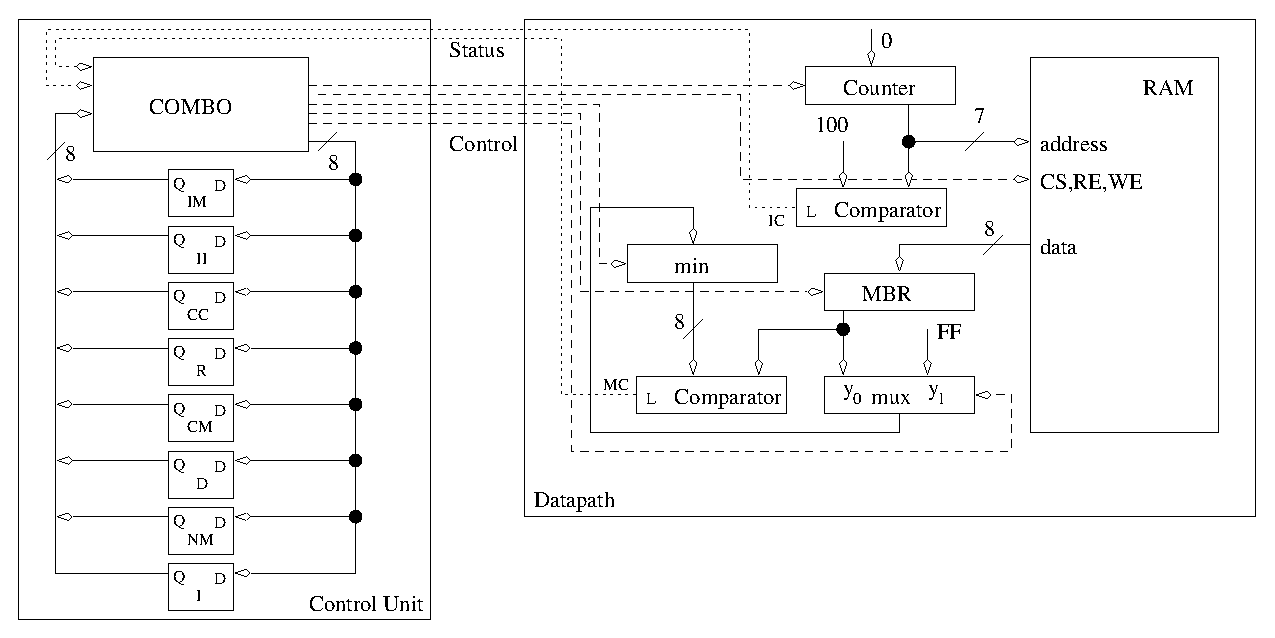
\includegraphics{../Fig/MinSearch2}} &
            \scalebox{0.3}{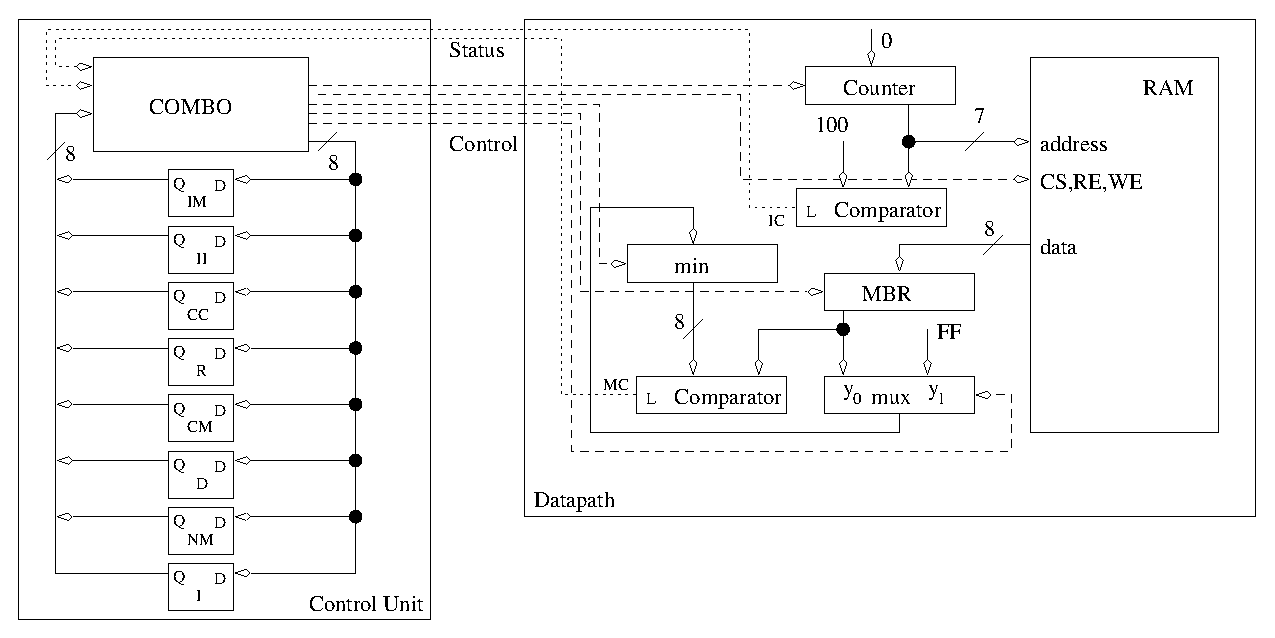
\includegraphics{../Fig/MinSearch2}} \\
            1. State \textbf{ InitMin} \vspace{10mm}        & 5. State \textbf{ CompM} \\
            \scalebox{0.3}{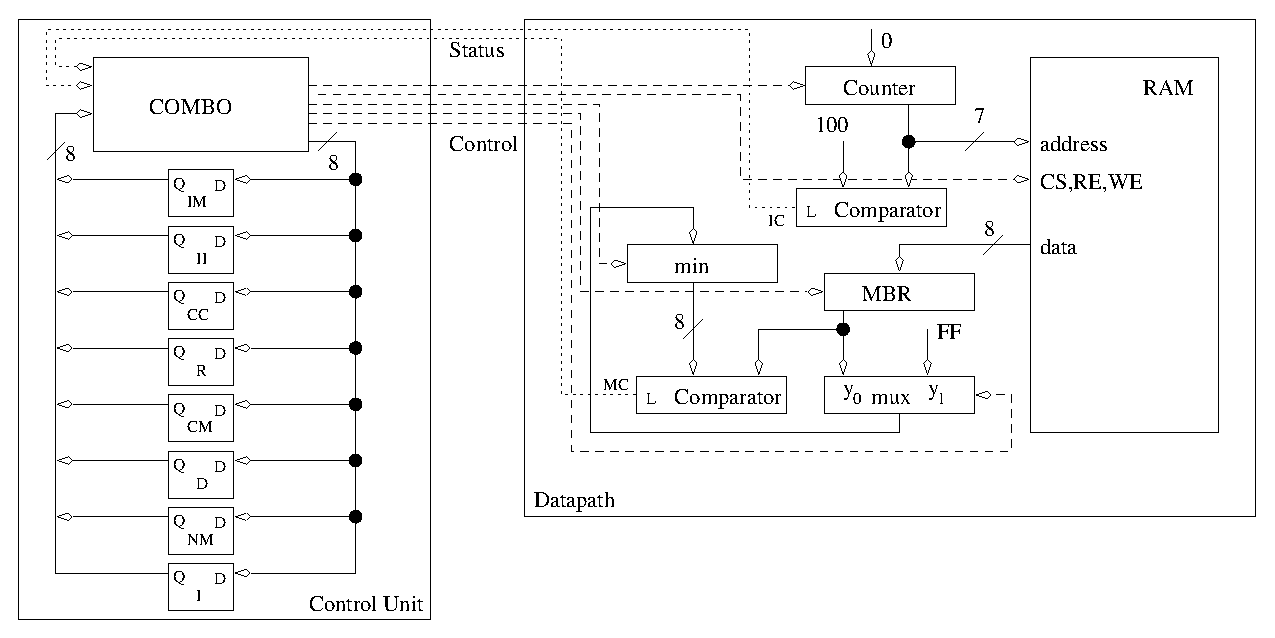
\includegraphics{../Fig/MinSearch2}} & i
            \scalebox{0.3}{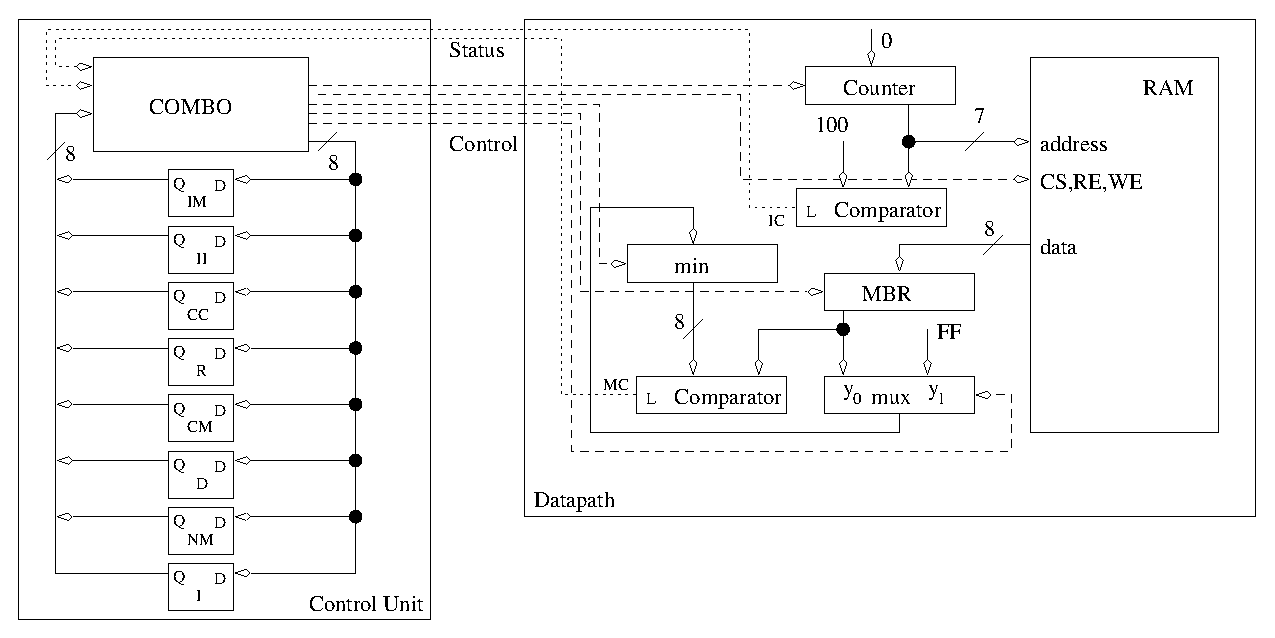
\includegraphics{../Fig/MinSearch2}} \\
            2. State \textbf{ InitI}   \vspace{10mm}        & 6. State \textbf{ NewMin} \\
            \scalebox{0.3}{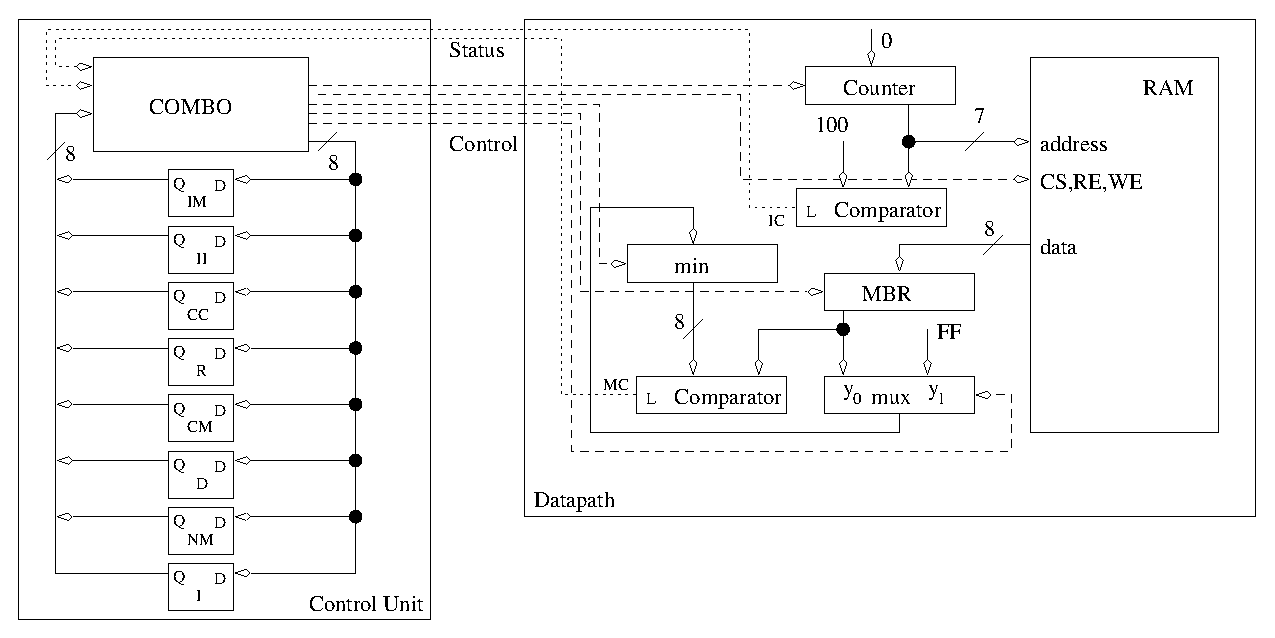
\includegraphics{../Fig/MinSearch2}} &
            \scalebox{0.3}{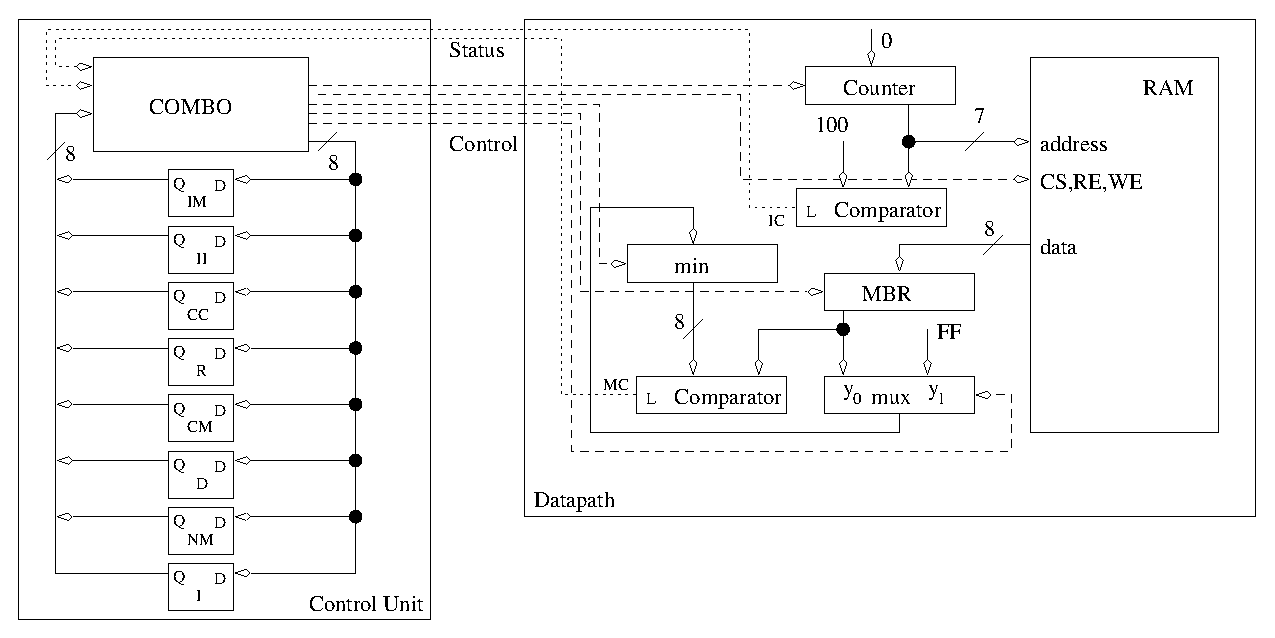
\includegraphics{../Fig/MinSearch2}} \\
            3. State \textbf{ CompC}   \vspace{10mm}          & 7. State \textbf{ Inc} \\
            \scalebox{0.3}{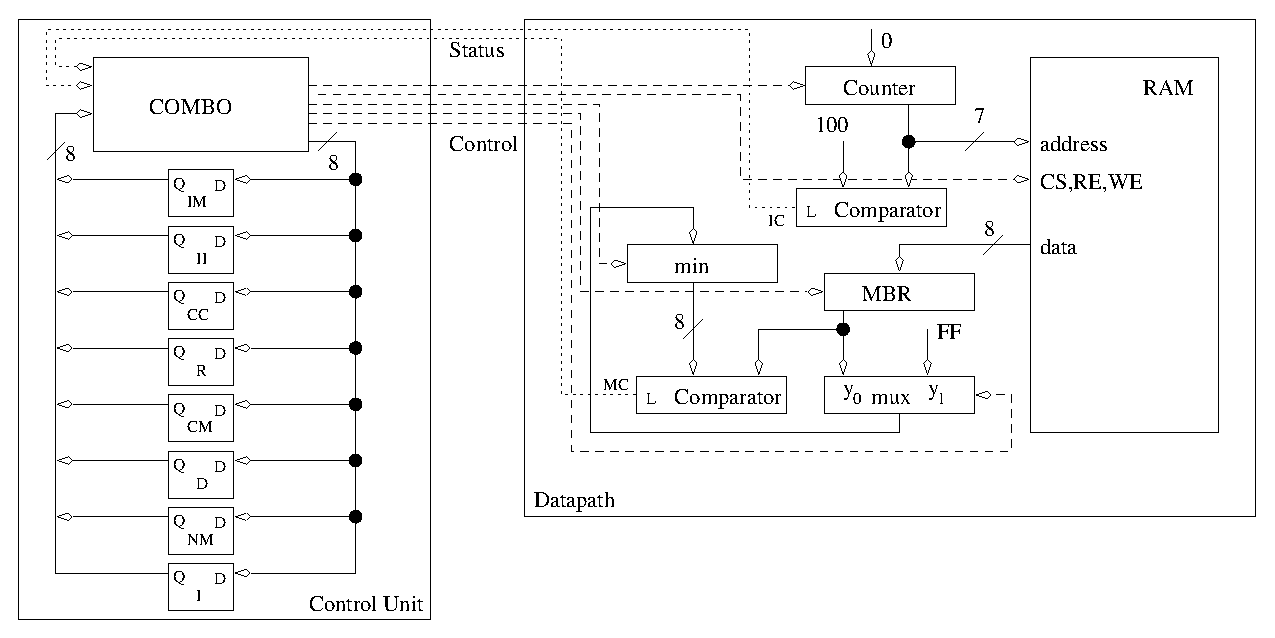
\includegraphics{../Fig/MinSearch2}} &
            \scalebox{0.3}{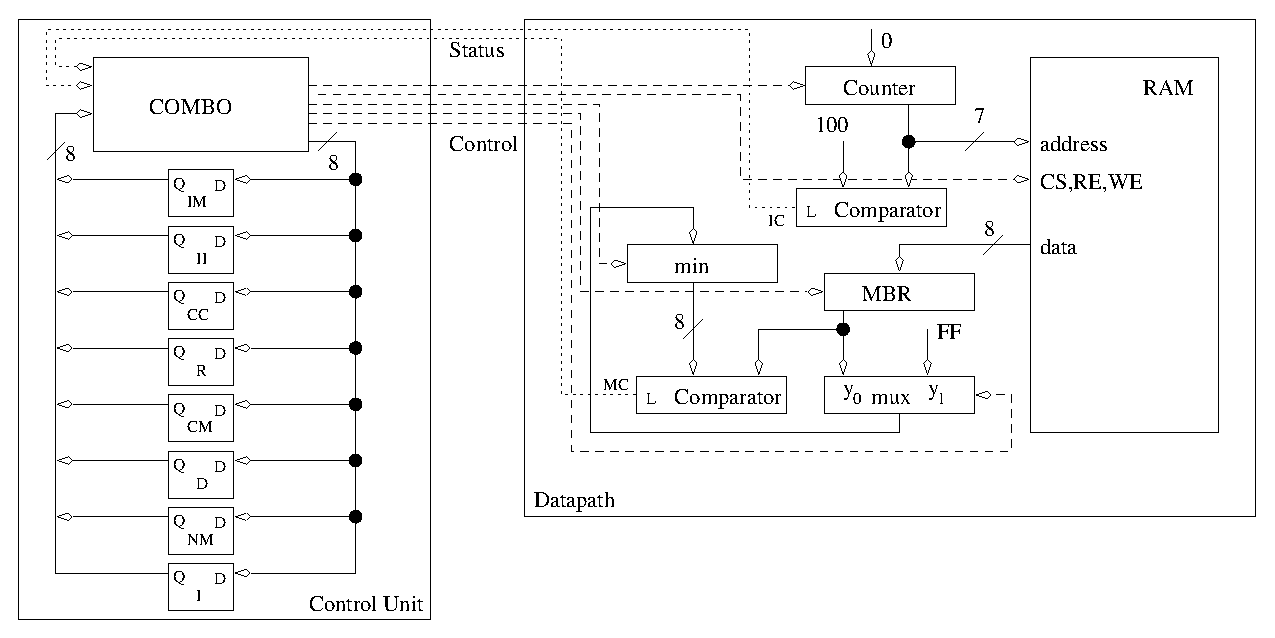
\includegraphics{../Fig/MinSearch2}} \\
            4. State \textbf{ Read}                                  & 8. State \textbf{ CompC} \\
        \end{tabular}

        \pagebreak

    \item[Bit Counter]
        Design a digital circuit that counts the number of 1's in an
        8 bit number X and puts the result into a register Y.
        The 8 bit number is provided by an external user using a two-line
        handshake protocol. The digital circuit is to play the role of the
        passive consumer.  Your circuit should do this task forever.  That
        is, after counting the number of 1's, you circuit should read
        in a new value of X.

\begin{verbatim}
1.  while(true) {               // Forever
2.      while(REQ==0);          // Wait for the REQ signal
3.      X = data;               // When we get a REQ latch data
4.      ACK = 1;
5.      while(REQ == 1);        // Wait for REQ to go low
6.      ACK = 0;                // then drop the ACK
7.      Y = 0;                  // Clear the bit count
8.      for (i=0; i<8; i++) {   // For each bit of X
9.          if (X(0) == 1) then // If the LSB of X is a 1
10              Y = Y + 1;      //   then increment Y
11          X = X >> 1;         // Shift X to the right 1 bit
12      } // end for
13  } // end while
\end{verbatim}

        \scalebox{0.7}{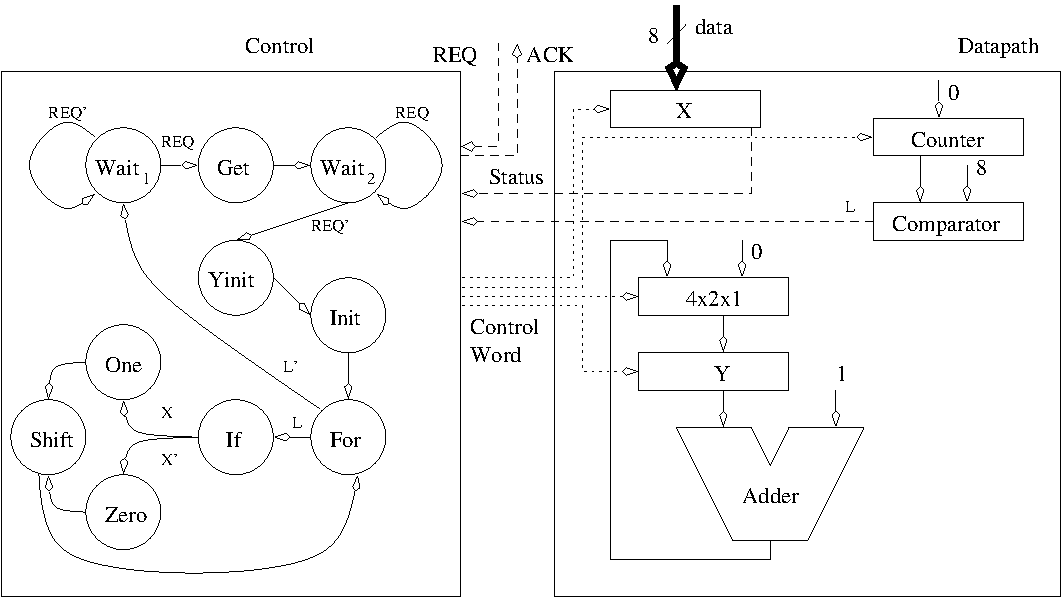
\includegraphics{../Fig/BitCount1}}

        \begin{tabular}{c||c|c|c|c|c}
            State   & ACK       &   X         &  Reg Y    & Y mux         & Counter       \\ \hline
            &           &   00 hold   &  0 hold   & 0 load 0      & 00 hold       \\ \hline
            &           &   01 lsr    &           &               & 01 load       \\ \hline
            &           &   10 lsl    &  1 load   & 1 load Add    & 10 count      \\ \hline
            &           &   11 load   &           &               &               \\ \hline \hline
            Wait1   &          &           &          &              &             \\ \hline
            Get     &          &           &          &              &             \\ \hline
            Wait2   &          &           &          &              &             \\ \hline
            Yinit   &          &           &          &              &             \\ \hline
            Init    &          &           &          &              &             \\ \hline
            For     &          &           &          &              &             \\ \hline
            If      &          &           &          &              &             \\ \hline
            One     &          &           &          &              &             \\ \hline
            Zero    &          &           &          &              &             \\ \hline
            Shift   &          &           &          &              &             \\
        \end{tabular}

        \begin{tabular}{p{2in}p{1in}}
            $D_{W1} =$    &    $Z_{ACK} =$          \\
            $D_{G} = $    &    $Z_{X} = $        \\
            $D_{W2} =$    &    $Z_{RegY} =$      \\
            $D_{YI} =$     &    $Z_{Ymux} =$         \\
            $D_{I} = $    &    $Z_{C1} =$         \\
            $D_{F} = $    &    $Z_{C0} =$         \\
            $D_{If} =$     &                \\
            $D_{One} =$     &                \\
            $D_{Zer} =$     &                \\
            $D_{Sft} =$     &                \\
        \end{tabular}

        \pagebreak

    \item[RAM counter]
        Build a circuit that reads in an 8 bit value, KEY, using a two
        line handshake; your circuit is a passive consumer.
        Your circuit should search an 8kx8 RAM counting the number
        of words that match KEY.  It takes one full clock cycle
        to read the RAM.  You may assume that the RAM is pre-loaded
        with data.  Your circuit should do this task forever.

\begin{verbatim}
1.    while(1) {
2.        while(REQ == 0);
3.        KEY = data;
4.        ACK = 1;
5.        while(REQ == 1);
6.        ACK = 0;
7.        match = 0;
8.        for(i=0; i<8191; i++) {
9.            MBR = RAM[i];
10.            if (MBR == KEY) {
11.                match=match+1;
12.            } // end if
13.        } // end for
14.    } // end while
\end{verbatim}

        \scalebox{0.5}{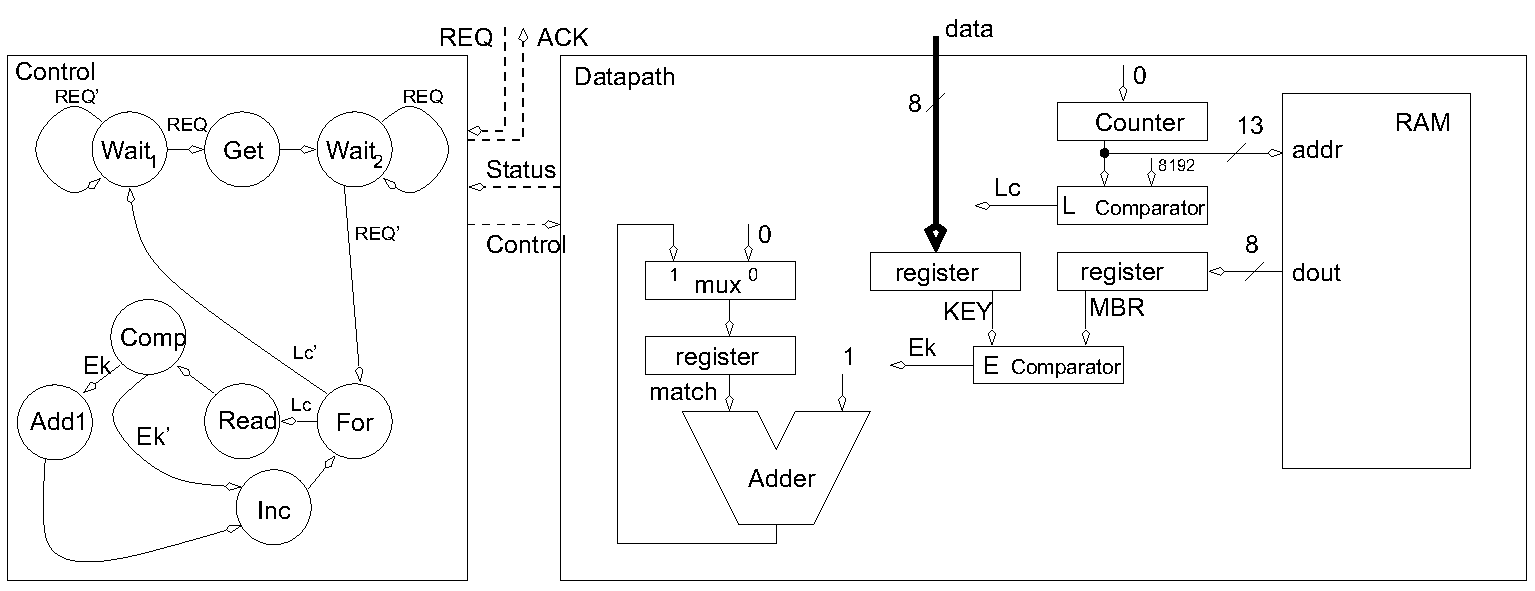
\includegraphics{../Fig/RAMmatch}}

        {\tiny
            \begin{tabular}{c||c|c|c|c|c|c|c}
                State   & ACK   & mux       &  Reg match& Reg KEY & Counter     & MBR    & enb             \\ \hline
                & 0     & 0 pass 0  &  0 hold   & 0 hold  & 00 hold     & 0 hold & 0      \\ \hline
                &       &           &           &         & 01 load     &        &               \\ \hline
                & 1     & 1 match+1 &  1 load   & 1 load  & 10 count    & 1 load & 1 read  \\ \hline \hline
                Wait1   &      &          &          &        &           &       &               \\ \hline
                Get     &      &          &          &        &           &       &             \\ \hline
                Wait2   &      &          &          &        &           &       &             \\ \hline
                For     &      &          &          &        &           &       &           \\ \hline
                Read    &      &          &          &        &           &       &             \\ \hline
                Comp    &      &          &          &        &           &       &             \\ \hline
                Add1    &      &          &          &        &           &       &        \\ \hline
                Inc     &      &          &          &        &           &       &            \\
        \end{tabular} }

        \pagebreak

    \item [Extra]
        Design a circuit that moves $M$ consecutive words from address $S$ (source) to
        address $D$ (destination).  For example, if $M=4$, $S=3EA$ and $D=1FE$ then the
        circuit would move words 3EA, 3EB, 3EC and 3ED to address 1FE, 1FF, 200 and 201.
        Each of $M,S,D$ is preloaded into a register.  While this problem appears simple,
        its really rather treacherous.  The circuit will have to handle cases where
        $S+M > D$.  In such a case the order of the data movement must be carefully planned.
        In order to simplify the design, assume that $S<D$.  Turn in an algorithm,
        datapath and control, the
        control word, MIEs and OEs.  These circuit will need a three-state buffer to
        be able to both read and write to the RAM.  Do not worry about the sizes of the
        registers or RAM.

    \item[Roulette]

        You are to construct a digital circuit that plays a game of
        roulette, allows betting and keeps track of total earnings.
        The roulette wheel has 8 slots, labeled $1 \ldots 8$.  The player
        can play one of the numbers straight or play even or odd.
        The player starts with \$10.
        The layout of the machine is shown in Figure~\ref{fig:Roulette}.
        \begin{figure}[ht]
            \center{\scalebox{0.5}{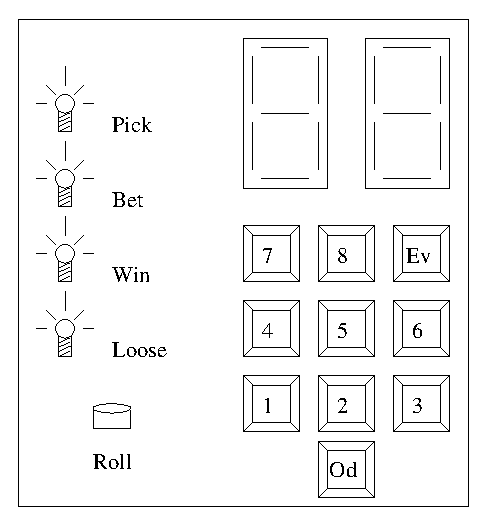
\includegraphics{../FigHw/Prob8-17}}}
            \caption{The layout of the roulette playing machine.
                The two 7 segment displays at the top are used for a variety
            of purposes.}
            \label{fig:Roulette}
        \end{figure}

        The sequence of events is as follows:
        \begin{enumerate}
            \item    The circuit lights up the PICK LED.
                The player enters their guess; a number between 1-8, even or odd.
                While holding down their guess they press the roll button.
            \item    The circuit displays the picked number in the left most
                7 segment display.  The circuit lights up the BET LED.
                The player enters a one digit bet between 1 to 8.  While holding
                down their bet they press the roll button.
            \item     The circuit displays the bet on the rightmost 7-segment
                display.
                The player pushes and holds down the roll button.
                The circuit increments a mod 8 counter while the roll
                button is depressed. It would be nice to display the
                current count value on right 7-seven segment display.
                Since the clock cycle is on the order of milliseconds,
                then the user would not be able to anticipate the roll.
            \item    The player releases the roll button.  The final roll
                is displayed on the rightmost 7-segment display.
                The circuit stops incrementing the counter and checks
                to see if the final value matches the players guess.
                If the match is correct then light the WIN LED and
                increment the players earnings.  If the match is incorrect
                then light the LOOSE LED and decrement the players
                earnings.
            \item    The play hits the roll button to clear the roll information
                from the 7-segment displays.
            \item    The circuit displays the players earnings on the 7-segment
                display.
            \item    When the user pushes the roll button then goto step 1.
        \end{enumerate}

        Set reasonable bounds on the maximum winnings.  Values may be displayed
        in hexadecimal (you may assume that you have a hex to 7-segment display
        converter at your disposal).
        \\
        \\

        \textbf {Algorthm}
        {\small
            \\
            1. cash = 10; \\
            2. LeftSeven = blank;     \\
            3. RightSeven = cash;     \\
            4. while(cash != 0) {     \\
                5.     LEDarray = 1 0 0 0;    // Pick Bet Win Loose     \\
                6.     while(ROLL == 0);     \\
                7.     guess = Datain;     \\
                8.     while(ROLL == 1);     \\
                9.          \\
                10.     LEDarray = 0 1 0 0;    // Pick Bet Win Loose     \\
                11.     LeftSeven = guess;     \\
                12.     RightSeven = blank;     \\
                13.     while(ROLL == 0);     \\
                14.     bet = Datain;     \\
                15.     while(ROLL == 1);     \\
                16.          \\
                17.     LEDarray = 0 0 0 0;    // Pick Bet Win Loose     \\
                18.     RightSeven = bet;     \\
                19.     while(ROLL == 0);     \\
                20.     while(ROLL == 1) count = count + 1;     \\
                21.      \\
                22.     RightSeven = count;     \\
                23.     if (count == guess) {     \\
                    24.         cash = cash + (bet *4);     \\
                    25.         LEDarray = 0 0 1 0;    // Pick Bet Win Loose     \\
                26.     } else {     \\
                    27.         cash = cash - bet;     \\
                    28.         LEDarray = 0 0 0 1;    // Pick Bet Win Loose     \\
                29.     }     \\
                30.     while(ROLL == 0);     \\
                31.     while(ROLL == 1);     \\
                32.     RightSeven = cash;     \\
                33.      \\
            34. }         \\
            35. LEDarray = 0 0 0 1;    // The user is out of money     \\
            36. while(1);        // Halt the machine     \\
        }

        \begin{landscape}
            \textbf{Datapath and Control}
            \begin{figure}[ht]
                %\center{\scalebox{0.7}{\includegraphics{./Sol8-16-blank}}}
            \end{figure}

            \pagebreak

            \textbf{ Control Word}

            \begin{table}
                \caption{The control word for the roulette circuit and its value for each state.}
                \label{table:roulette}
                {\small
                    \begin{tabular}{l|l|l|l|l|l|l|l|l|l|l}

                        State &  counter& guess  & bet    & cmux      & bmux     & cash   & add/sub & ledmux
                        & rmux   & lmux \\ \hline
                        & 00 hold & 0 hold & 0 hold & 0 \$10    & 0 bet    & 0 hold & 0 add  & 00 (pick) &00
                        cash &00 cash  \\ \hline
                        & 01 load & 0 load & 1 load & 1 add/sub & 1 bet<<2 & 1 load & 1 sub  & 01 (bet ) &01
                        bet  &01 guess \\ \hline
                        & 10 up   &        &        &            &          &        &        & 10 (win ) &10
                        count&10 blank \\ \hline
                        &         &        &        &            &          &        &        & 11 (loose)&11
                        blank&         \\ \hline
                        &         &        &        &            &          &        &        &          &
                        &   \\ \hline
                        init  &       &       &       &           &         &       &       &        &       & \\ \hline
                        wg1   &       &       &       &           &         &       &       &        &       & \\ \hline
                        guess &       &       &       &           &         &       &       &        &       & \\ \hline
                        wg2   &       &       &       &           &         &       &       &        &       & \\ \hline
                        wb1   &       &       &       &           &         &       &       &        &       & \\ \hline
                        bet   &       &       &       &           &         &       &       &        &       & \\ \hline
                        wb2   &       &       &       &           &         &       &       &        &       & \\ \hline
                        wr1   &       &       &       &           &         &       &       &        &       & \\ \hline
                        spin  &       &       &       &           &         &       &       &        &       & \\ \hline
                        load 1&       &       &       &           &         &       &       &        &       & \\ \hline
                        comp  &       &       &       &           &         &       &       &        &       & \\ \hline
                        win   &       &       &       &           &         &       &       &        &       & \\ \hline
                        add   &       &       &       &           &         &       &       &        &       & \\ \hline
                        loose &       &       &       &           &         &       &       &        &       & \\ \hline
                        sub &       &       &       &           &         &       &       &        &       & \\ \hline
                        wn    &       &       &       &           &         &       &       &        &       & \\
                    \end{tabular}
                }
            \end{table}
        \end{landscape}

    \item[Light Show]

        A light show consists of an endlessly repeating sequence of up to 16 frames.
        A frame is an illuminated pattern of LEDs on a LED bar graph. The user
        creates a light show by specifying the number of frames in the show, editing
        those frames, and then instructing the circuit to cycle through the frames.
        The input to the circuit comes from a standard PS/2 keyboard. The output of
        the circuit is displayed on a LED bar graph and a 7-segment display. The
        behavior of the Light Show circuit is given in Figure~\ref{fig:LSbehavior}.

        \begin{figure}[ht]
            \center{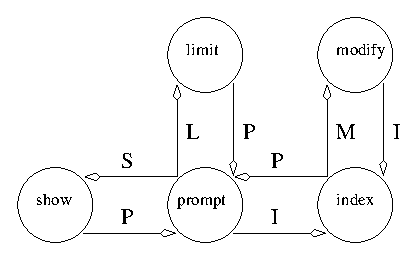
\includegraphics{../Fig/Behavior}}
            \caption{A state diagram describing the behavior of the Light Show circuit.}
            \label{fig:LSbehavior}
        \end{figure}

        The Light Show circuit changes state when the users presses a key on
        the keyboard. For example, pressing ``M" while in the \textbf{ index } state causes
        the circuit to transition into the \textbf{ modify state}. The behavior of the
        Light Show circuit in each of its states is described in
        Table~\ref{table:LSbehavior}.

        \begin{table}
            \begin{tabular}{l|p{0.5in}|p{0.5in}|p{2.0in}}
                \textbf{ State }    & LED bar graph    & 7-segment    & Behavior                 \\ \hline \hline
                \textbf{ reset }    & blank        & blank        & All sequential elements are reset     \\ \hline
                \textbf{ prompt }    & blank        & ``P"        & Waiting for user input        \\ \hline
                \textbf{ limit }    & blank        & current limit    & The number of frames in the light show is called
                the limit. If the user enters a hex value between 0-F it is stored as the new limit. \\  \hline
                \textbf{ index }    & current frame    & current index    & Each frame in the show has an
                index which defines
                its position in the show. If the user enters a hex value between 0-F, this frame will
                be edited in the \textbf{ modify } state.                         \\ \hline
                \textbf{ modify }    & current frame    & current index    & Each frame has eight bits which
                specify the state of
                the 8 LEDs on the bar graph.  These bits are toggled by pressing the corresponding
                key. For example, if LED 5 is on, pressing ``5", causes LED 5
                to go off.                                \\ \hline
                \textbf{ show }    & cycle through frames & current index & Consecutive frames are displayed on the
                LED bar graph at around 4Hz. After the last frame is displayed, the circuit loops
                back to the 0th frame.                             \\
            \end{tabular}
            \caption{The behavior of the Light Show circuit in each of its states.}
            \label{table:LSbehavior}
        \end{table}

        The algorithm for the light show circuit continually scans the busy signal
        and the keyboard scan code.  When the user presses either a ``L",
        ``I", or ``S",
        the algorithm drops into one of the subfunctions described in
        Table~\ref{table:LSbehavior}.  Assume the Light Show circuit is
        clocked at 16MHz.  The clock rate is needed in order to create a delay of
        0.25 seconds required to pace the frames during the show phase.

        \pagebreak
\begin{verbatim}
1.  while(1) {
2.      HexDisplay = "P"
3.      if (!busy and IsL(ScanCode)) {
4.          while (!busy' and !IsP(ScanCode)) {
5.             HexDisplay = Hex2Seven(limit);
6.             BarGraph = 0x00;
7.             if (!busy and IsHex(ScanCode)) {
8.                  limit = Scan2Hex(ScanCode);
9.                  while(!busy);
10.     }   }  }

11.     if (!busy and IsI(ScanCode)) {
12.         while (busy or !IsP(ScanCode)) {
13.             HexDisplay = Hex2Seven(index);
14.             if (!busy and IsHex(ScanCode)) {
15.                index = Scan2Hex(ScanCode);
16.                 while(!busy);
17.             }

18.             if (!busy and IsM(ScanCode)) {
19.                 while (busy or !IsI(ScanCode)) {
20.                     HexDisplay = Hex2Seven(index);
21.                     BarGraph = RAM[index];
22                         while(!busy);
23                         while(busy);
24.                     if (!busy and IsOct(ScanCode)) {
25.                         RAM[index] = Flip(IsOct(ScanCode),RAM[index]);
26.     }   }   }   }   }

27.     if (!busy and IsS(ScanCode)) {
28.        index = 0;
29.         while(!busy and !IsP(ScanCode)) {
30.             BarGraph = RAM[index];
31.             HexDisplay = Hex2Seven(index);
32.             for (timer=0; timer<2^22; timer++);
33.             index += 1;
34.             if (index == limit) index=0;
35.  }  }
\end{verbatim}

        \begin{landscape}
            \begin{figure}[ht]
                %\center{\scalebox{0.9}{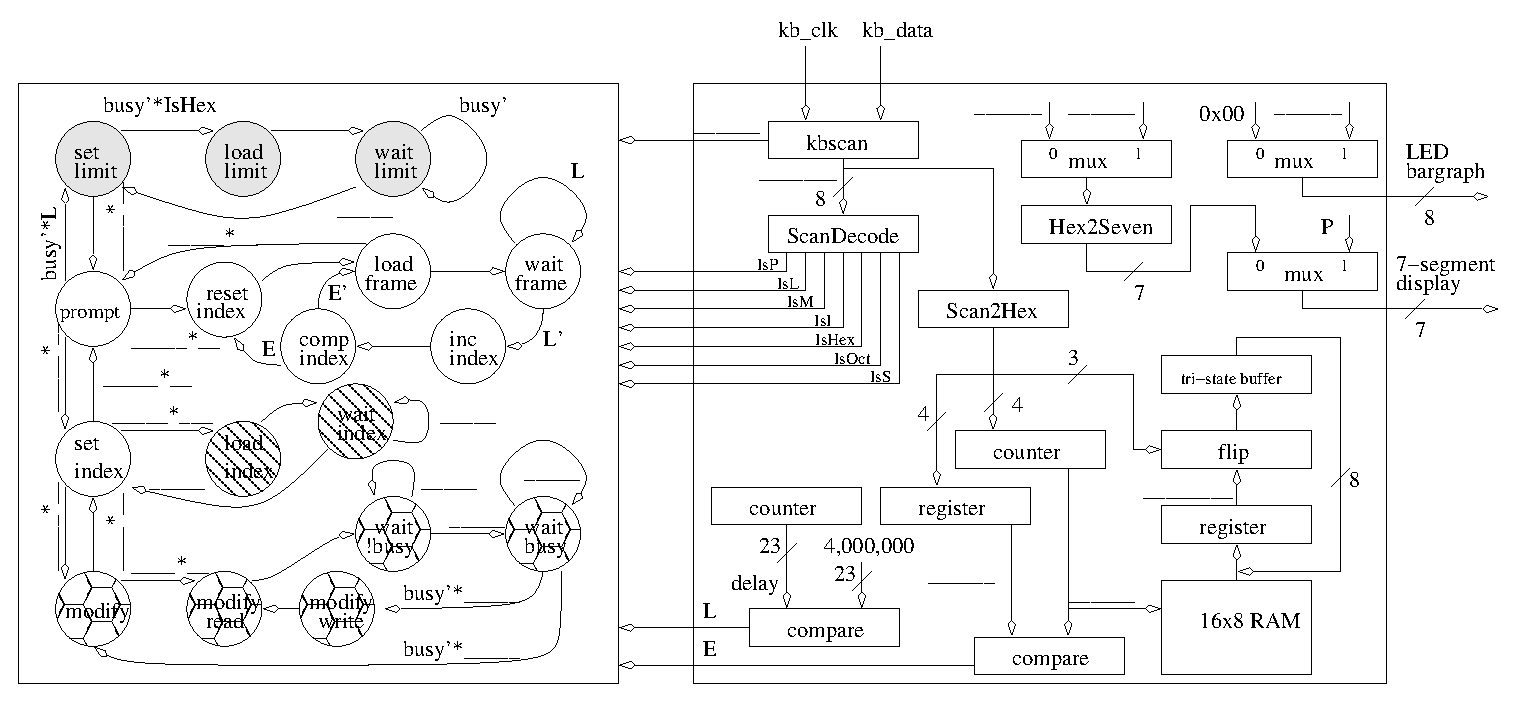
\includegraphics{./LightShowCir-hand}}}
                \caption{The datapath and control for the Light show circuit.}
                \label{fig:LightShowCir}
            \end{figure}

            \begin{table}
                {\small
                    \begin{tabular}{c||c|c|c|c|c|c|c|c|c|c|c}
                        \textbf{ State }     & bar & 7-seg & hex & index & delay & limit    & bargraph & CS &
                        R/W' & tsb & flip \\
                        & mux & mux   & mux & count & count & register & register &       &       & &
                        \\  \hline \hline
                        & 0 0x00 & 0 index & 0 7-seg & 00 hold & 00 hold & 0 hold & 0 hold & 0 off & 0 write
                        & 0 tri & 0 pass \\
                        & 1 bar    & 1 limit & 1 ``P"& 01 cnt & 01 cnt & 1 load &    1 load & 1 on    &  1
                        read & 1 pass & 1 flip \\
                        &     &     &     & 10 load & 10 load & & & & & \\
                        &     &     &        & 11 reset    & 11 reset & & & & \\ \hline \hline
                        \textbf{ prompt }      &       &      &      &       &       &      &      &      &
                        &      &   \\ \hline
                        \textbf{ set limit }  &       &      &      &       &       &      &      &      &
                        &      &   \\ \hline
                        \textbf{ load limit } &      &      &      &       &       &      &      &      &   &
                        &   \\ \hline
                        \textbf{ waitlimit } &      &      &      &       &       &      &      &      &   &
                        &   \\ \hline
                        \textbf{ reset inde  } &      &      &       &       &       &      &      &      &
                        &      &   \\ \hline
                        \textbf{ load frame } &      &      &      &       &       &      &      &      &   &
                        &   \\ \hline
                        \textbf{ wait frame } &      &      &      &       &       &      &      &      &   &
                        &   \\ \hline
                        \textbf{ inc index } &      &      &      &       &       &      &      &      &   &
                        &   \\ \hline
                        \textbf{ comp index } &      &      &      &       &       &      &      &      &   &
                        &   \\ \hline
                        \textbf{ set index } &      &      &      &       &        &      &       &      &
                        &      &   \\ \hline
                        \textbf{ load index } &      &      &       &       &       &      &      &      &
                        &   &   \\ \hline
                        \textbf{ wait index } &      &      &      &       &       &      &      &      &   &
                        &   \\ \hline
                        \textbf{ modify    } &      &      &      &       &       &      &      &      &   &
                        &   \\ \hline
                        \textbf{ modify read} &      &      &      &       &       &      &      &      &   &
                        &   \\ \hline
                        \textbf{ modify write } &      &      &      &       &       &      &      &       &
                        &      &   \\ \hline
                        \textbf{ wait !busy } &      &      &      &       &       &      &      &      &   &
                        &   \\ \hline
                        \textbf{ wait busy } &      &      &      &       &       &      &      &      &   &      &   \\
                    \end{tabular}
                }
                \caption{The control word for the LightShow circuit and its value for each state.}
                \label{table:LightShow}
            \end{table}

        \end{landscape}

\end{description}
